% editing notes: don't use auto-fill-mode

\documentclass[man,floatsintext]{apa6}
\usepackage{amsmath}
\usepackage{amssymb}
\usepackage{graphicx}
\usepackage{geometry}
\usepackage{hyperref}
\usepackage[natbibapa]{apacite}
\usepackage{times}
\usepackage{multirow}
\usepackage{color}
\usepackage{array}
\usepackage{verbatim}


\newcommand{\tcite}[1]{$\langle${\footnotesize \texttt{#1}}$\rangle$}

% add key-bindings for bold and italic
% the (interactive) bit is crucial, HT http://stackoverflow.com/a/14635806/351392
\begin{comment}
  (local-set-key (kbd "s-b") (lambda ()  (interactive) (TeX-font nil ?\C-b)))
  (local-set-key (kbd "s-i") (lambda ()  (interactive) (TeX-font nil ?\C-e)))
\end{comment}

\graphicspath{{images/}}

\shorttitle{Semantic coherence and distributional learning}
% \shorttitle{}
\title{Semantic coherence facilitates distributional learning}
\author{Long Ouyang, Lera Boroditsky, Michael C. Frank}
\affiliation{Department of Psychology, Stanford University\vskip 5em Word count: 6,706}

\authornote{An earlier version of this paper appeared in the Proceedings of the 34th Annual Meeting of the Cognitive Science Society. Address correspondence to:\\
Long Ouyang~\\
Jordan Hall, Building 01-420\\
450 Serra Mall\\
Stanford, CA, 94305\\
Email: \texttt{longouyang@post.harvard.edu}}

\abstract{Computational models have shown that purely statistical knowledge about words' linguistic contexts is sufficient to learn many properties of words, including grammatical category and meaning. For example, a learner might infer that ``postman'' and ``mailman'' are similar because they have quantitatively similar patterns of association with \emph{other} words (e.g., both ``postman'' and ``mailman'' tend to occur with words like ``deliver'', ``truck'', ``package''). Are people able to use distributional statistics in learning language? Results from prior artificial language learning experiments suggest that the answer may be no. However, experiments in this paradigm expose participants to entirely novel words, whereas real language learners encounter input that contains some known words that are semantically organized. In three experiments, we show that (1) the presence of familiar semantic reference points facilitates distributional learning and (2) this effect crucially depends both on the presence of known words and the adherence of these known words to some semantic organization.}

\keywords{distributional learning; word learning; semantic coherence}

\begin{document}
\maketitle

\begin{quote}
``\emph{You shall know a word by the company it keeps.}'' Firth (1957, p.11)
\end{quote}

How do people learn language? Research indicates that learners use many information sources, including physical, social, conceptual, and linguistic cues \citep{clark1988, markman1991, gleitman1990, baldwin1993, hollich2000}. In addition to external sources of information, the distributional properties of language itself can be informative about both its structure and meaning. A wide variety of experiments show that learners are sensitive to these distributional properties. For example, learners can group sounds together into word forms based on their statistical co-occurrence \citep{saffran1996a, saffran1996b} and pair word forms with their referents based on consistent associations \citep{yu2007,smith2008}. In the current paper, we explore a more sophisticated type of distributional learning: learning about a word using evidence about the linguistic contexts that it occurs \citep{smith1966, maratsos1980, braine1987, redington1998}.

As an example of distributional learning, one might infer that ``postman'' and ``mailman'' have similar meanings or are similar parts of speech based solely on the fact that they both tend to occur with words like ``deliver'', ``package'', and ``truck'' in comparable configurations and frequencies. To give an intuition in a different domain, we might judge whether two people are similar based on their patterns of association with other people. If we know that Alice associates with professors and college sophomores and that Bob associates with accountants and lawyers, we might judge that they are dissimilar. For words, this kind of learning is driven not by \emph{direct} co-occurrence between two words of interest but rather by the similarity in their linguistic contexts---their patterns of co-occurrence with \emph{other} words. As \citet{firth1957} put it, one learns a word ``by the company it keeps'' (p.11). We will refer to learning from such learning as \emph{distributional learning}.

Distributional learning is a general mechanism thought to be important throughout language learning, including acquisition of word meaning \citep{landauer1997} and grammatical category \citep{redington1998}. Nevertheless, a number of experiments, conducted mainly on acquisition of grammatical category, suggest that human learners' capacities are limited in this regard \citep{braine1987, brooks1993, frigo1998, kempe2001, gerken2005, frank2011}.

Our study addresses this mismatch by specifying conditions under which people succeed in distributional learning. In particular, we investigate the effect of existing linguistic knowledge. Prior experiments typically exposed learners to artificial languages composed of entirely novel words. Our experiments suggest that \emph{semantic coherence}, the presence of known words adhering to some semantic organization, facilitates distributional learning. Put another way, a small semantic hook allows people to better leverage distributional information for learning. Phrased in terms of the Alice--Bob example, we stand a better chance of learning about Alice from her associates if those associates play roles that are already meaningful to us. Knowing that Alice associates with professors and college sophomores gives us a clearer picture of her than, say, knowing that she associates with taphonomists and bryologists.\footnote{Though, we can infer much more about Alice if we know that taphonomy is the study of decay and fossilization and that bryology is the study of certain plants called bryophytes, which include mosses, hornworts, and liverworts.} Learning a word from its company is easier if this company is already familiar. 

We begin by briefly reviewing some of the computational evidence for distributional learning. We then introduce the specific language structure, MNPQ, that we explore in this paper. Next, we discuss research that uses the MNPQ structure to study distributional learning of grammatical categories. In Experiment 1, we present evidence that semantic coherence can facilitate distributional learning and that learners make use of acquired distributional information when performing an online referent assignment task. In Experiments 2 and 3, we further explore this effect by isolating two components of semantic coherence---familiarity of words and presence of an overarching semantic organization ---and find that neither alone facilitates learning. We conclude by discussing the limitations of purely artificial language learning, possibilities for future empirical and computational work, and potential mechanisms for the effects we observe.
 
\subsection{Computational evidence for distributional learning}

Initial proposals about distributional learning came from philosophical and linguistic research on the nature of meaning. In the philosophical literature, \citet{wittgenstein1953} objected to the idea that words have precise, formal definitions and argued that meaning derives from patterns of usage. To illustrate, he considered the word ``game'' -- a term used to describe activies as varied as chess, poker, basketball, the Olympics and so forth -- and observed that these activities lack a shared essence that we could distill to a definition. To use a spatial metaphor, the set of things called games does not appear to be a contiguous region that we could draw a boundary for, but rather a ``complicated network of similarities overlapping and crisscrossing'' (\S 66). Wittgenstein argued that understanding meaning requires describing usage.

In linguistics, \citet{firth1957} similarly argued for a theory of meaning based on patterns of ``habitual collocation.'' For example (p.12), he asserts that part of the meaning of the ``cow'' is its co-occurrence with  ``milk'', as in ``They are milking the cows'' or ``Cows give milk.'' ``Tigress'' and ``lioness'' do not co-occur with ``milk'' as often and thus must differ somewhat in meaning. Firth stressed the utility of \emph{pure} co-occurrence independent of extralinguistic or even grammatical aspects. He even outlined a prescient kind of cluster analysis quite similar to modern-day statistical approaches:

\begin{quote}
``In the study of selected words, compounds and phrases in a restricted language for which there are restricted texts, an exhaustive collection of collocation will suggest a small number of groups of collocations for each word studied. The next step is the choice of definitions for meanings suggested by the groups'' (p. 13)
\end{quote}
Firth's contemporary Harris advanced a quantitative version of this notion called the \emph{distributional hypothesis}, which proposes that words are semantically similar to the degree that they participate in the same contexts \citep{harris1951}. Harris argued that, even in cases where word meaning was determined by extralinguistic influences, such influences would have distributional correlates. Thus, meaning could be divined by the quantitative analysis of purely linguistic information.

These proposals about the distributional theory of meaning stimulated early empirical work with humans, which typically supported the distributional hypothesis using small samples of human judgments and corpora \citep{rubenstein1965, clark1968, stefflre1971, geffroy1973, berryrogghe1973, szalay1974}. For example, \citet{rubenstein1965} compared synonym judgments for pairs of concrete nouns generated by one group of subjects with co-occurrence statistics in a corpus generated by a separate group of subjects. They found a positive relationship between synonymy and degree of linguistic context match.

\begin{figure}[t]
  \begin{center}
    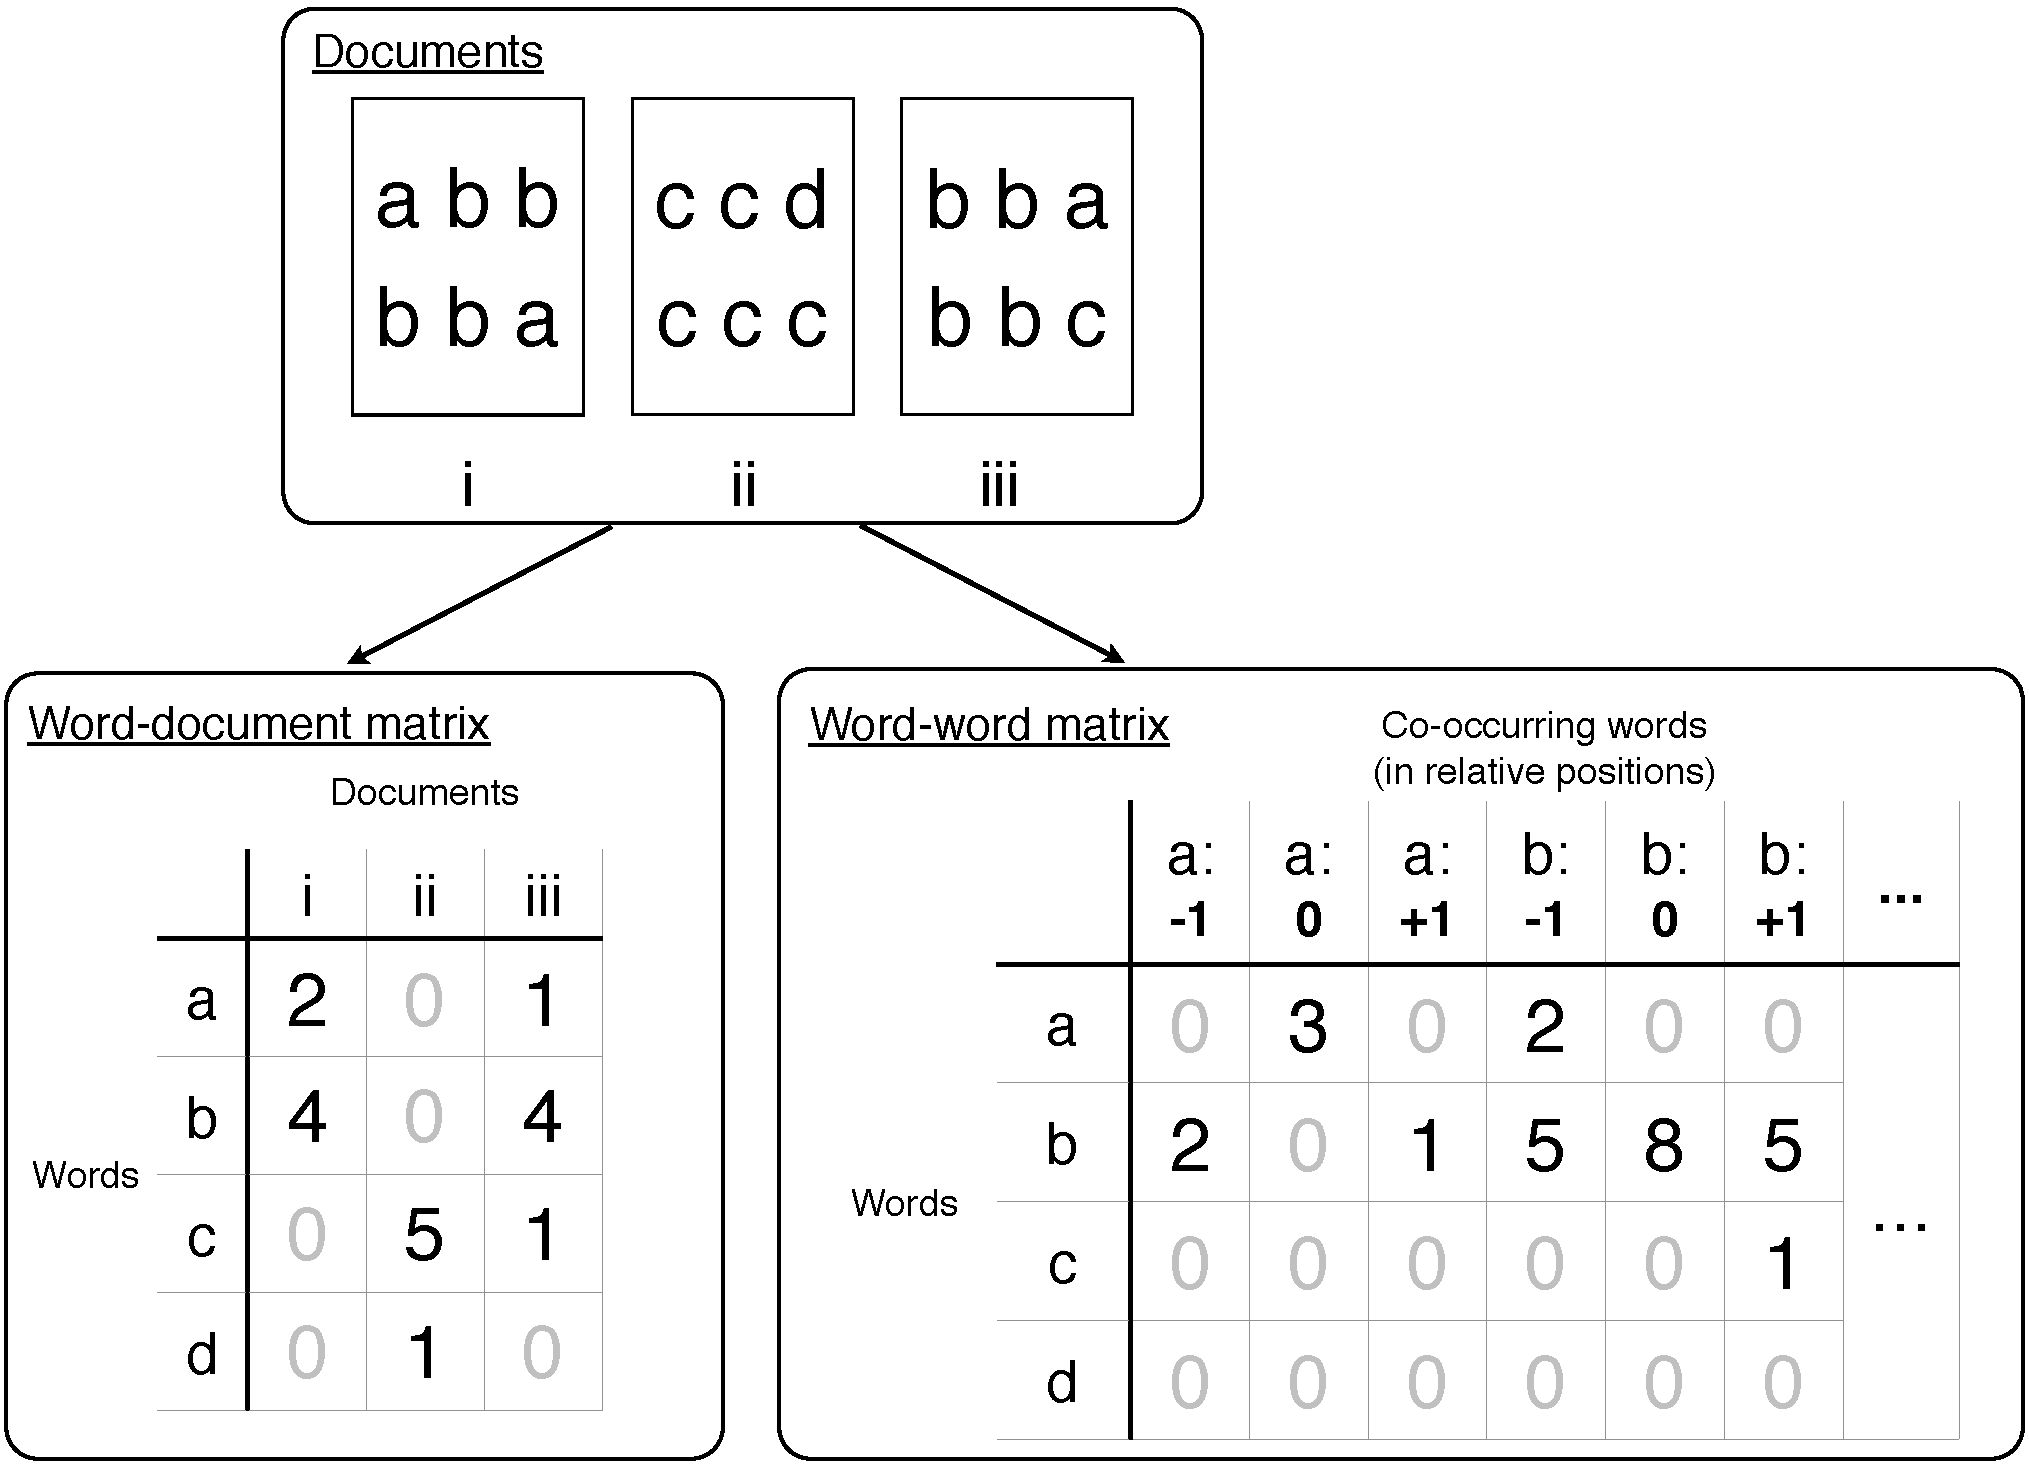
\includegraphics[width=0.9\linewidth]{matrices}
  \end{center}
  \caption{Word-document and word-word matrices. Word-document matrices measure how often words occur in particular documents. Word-word matrices measure how often pairs of words occur in certain relative positions.}
  \label{matrices}
\end{figure}

In the 1980s, computer scientists devised techniques that paved the way for large scale investigations of distributional learning. Motivated by practical issues in the field of information retrieval, they considered the relationships between words and documents. A typical problem was to retrieve documents relevant to a user query with certain search terms (i.e., a search engine). One solution to this problem is to represent documents as points in a high dimensional space whose dimensions are frequencies for different words \citep{salton1983}. This approach lends itself quite naturally to a matrix representation with words labeling rows, documents labeling columns, and cells encoding how often a particular word occurs in a particular document (Figure \ref{matrices}). While we can interpret such matrices as representing documents in terms of their component words, we can also interpret them representing words in terms of their frequency of use across different documents (a useful form for distributional learning). To make an analogy with our Alice--Bob example, such \emph{word-document} matrices license inferences about Alice and Bob based on \emph{where} they appear (rather than \emph{who} they appear with).

Note, however, that this representation discards information about the relative position of words within documents. The \emph{word-word} approach retains this information \citep{church1990, schutze1992}, labeling both rows and columns with words; a row might represent the meaning of word A and the count in a particular column might indicate frequency that word A occurred 2 words before word X (Figure \ref{matrices}). This corresponds to the initial example of inferences about Alice and Bob based on \emph{who} they appear with.

Computational models operating on such co-occurrence representations can acquire both semantic and syntactic properties of words. In the domain of semantics, \citet{landauer1997} built a word-document matrix from a corpus of encyclopedia articles, applied a dimensionality reduction technique (singular value decomposition), and computed the similarity between words using a cosine measure. This Latent Semantic Analysis model (LSA) was able to successfully pass a TOEFL synonym test. In the domain of syntax, \citet{redington1998} developed a model that performs hierarchical clustering on a word-word matrix to that successfully acquires grammatical categories like noun, verb, and adjective. In fact, these results suggest that co-occurrence statistics may be particularly powerful, offering leverage on many kinds of linguistic information. Although devised to learn grammatical categories, the model often learned clusters that had semantic organization. For example, in the cluster of adjectives, color words and number words formed separate clusters (p448).

The success of this early computational work led to a proliferation of models that learn from co-occurrence statistics (see \citealp{riordan2010} for an overview and comparison of state-of-the-art models). The computational evidence is quite suggestive: in principle, statistical patterns of co-occurrence can facilitate learning. However, while suggestive, this work is only indirect evidence of distributional learning. Researchers studying acquisition of grammatical categories have employed methods that can in principle provide stronger evidence. These studies expose learners to artificial languages with certain co-occurrence regularities and measure whether learners form categories on the basis of these regularities. In the next section, we discuss results of studies that have examined one co-occurrence structure called the MNPQ language.

\subsection{A puzzle: the MNPQ language}

The MNPQ language contains four categories of words, M (which includes $m_1$, $m_2$, and $m_3$), N ($n_1$, $n_2$, $n_3$), P ($p_1$, $p_2$, $p_3$), and Q ($q_1$, $q_2$, $q_3$). Participants hear two types of training sentences\footnote{ We use the term ``sentence'' following its meaning in formal language theory, where it refers to a sequence of symbols derived from a formal gramar. The sentences we examine in our work are clearly impoverished relative to real sentences found in natural languages.}: MN and PQ. Thus, sentences like $m_1 n_3$ are grammatical while sentences like $m_1 q_3$ are illegal. Early investigations \citep{braine1966, smith1966} found that participants tend to endorse novel grammatical sentences as familiar. However, participants also endorse ungrammatical MQ and PN sentences, suggesting that they learn position regularities (that M/P come first and N/Q come second) but not co-occurrence regularities (that M co-occurs with N but not Q and that P occurs with Q but not N). This failure to learn categories on the basis of pure co-occurrence has been reliably observed in a number of studies \citep{braine1987, brooks1993, frigo1998, kempe2001, gerken2005, lany2010, frank2011}. However, \citet[Experiment 5]{reeder2009} report successful learning of a related language, (Q)AXB(R). In this language, there are optional Q and R categories that serve to deconfound co-occurrence regularities from positional regularities (i.e., in MNPQ, Ms and Ps are always sentence-initial and Ns and Qs are always sentence-final). Thus, this work by \citeauthor{reeder2009} suggests that positional regularities may override co-occurrence regularities in the MNPQ language. Nevertheless, the MNPQ failures are puzzling, given that computational models suggest that distributional learning is a powerful mechanism.

MNPQ learning is possible, however, when co-occurrence information is partially or completely correlated with another cue. For example, \citet{braine1987} found successful MNPQ learning when co-occurrence information is partially correlated with natural gender. In this experiment, participants acquired an artificial language by learning to name pictures of referents. In the experimental condition, all pictures of men were labeled by Ms and all pictures of women were labeled by Ps (though not all Ms referred to men and not all Ps referred to women). Learning of the co-occurrence regularities was significantly higher in the experimental condition than in a control condition where natural gender was not correlated with M/P membership. Though Braine's experiment combined co-occurrence cues with natural gender, he suggested that phonological cues might better serve real-world language learners. For instance, Spanish and Italian speakers might learn grammatical gender categories by taking advantage of the fact that feminine nouns often end with \emph{-a}, while masculine nouns often end with \emph{-o}. More generally, demonstrations that co-occurrence information can be useful in concert with other information sources have encouraged researchers to study how disparate sources might be integrated to facilitate learning (e.g., \citealp{monaghan2005, johns2012}).

Nearly all of this empirical work has interpreted the results of human experiments with reference to learning grammatical category. To our knowledge, only one study has examined word meaning. Recently, \citet{lany2010} investigated Braine's proposal of correlating co-occurrence and phonological cues in a study of meaning acquisition. They found that 22-month old infants successfully learned an MNPQ language when co-occurrence was aligned with the number of syllables in a word (in particular, when N words were disyllabic and Q words were monosyllabic) but \emph{not} when the number of syllables was not predictive of N/Q membership. This suggests that distributional information may play a common role in acquisition of grammatical category and word meaning, at least for the MNPQ language. 

In our current work, we add to the literature on distributional learning by exploring a new information source: semantic coherence. To date, all studies have used the artificial language learning paradigm, with a vocabulary consisting of all novel words. Thus, at the beginning of the experiments, learners did not know the meanings of any of the words. Real learners, by contrast, typically know the meanings of some (if not most) words they hear and such words tend to relate to a single topic of discourse. Put another way, the language that real learners encounter tends to have semantic coherence; some words are known and adhere to some semantic organization. We ask: does semantic coherence facilitate distributional learning?

To explore this possibility, we presented participants with an MNPQ language where sentences took the form ``M and N'' or ``P and Q''. Note that we used the explicit English conjunction ``and'' between the two words, which imbued sentences with some semantic content (i.e., our stimuli were not merely a syntactic ordering). We hypothesized that a sufficient level of semantic coherence (specifically, a taxonomic coherence where Ms are animals and Ps were vehicles) would yield successful distributional learning for N and Q words. For instance, hearing the four sentences:
\begin{enumerate}
\item dog and dax
\item dog and ziv
\item car and wug
\item car and pif
\end{enumerate} might allow learners to infer that daxes and zivs are similar, as both words co-occur with ``dog'', and that wugs and pifs are similar, as both words co-occur with ``car.''

In Experiment 1, we tested whether semantic coherence facilitated distributional learning and whether learners might use distributional information to make inferences about word meaning. In Experiment 2, we compared semantic coherence to phonological coherence. In Experiment 3, we compared semantic coherence to a semantic baseline that used known words that did not adhere to any obvious semantic organization.

\section{Experiment 1: Semantic Coherence}

In all the experiments reported in this paper, we exposed participants to auditory sentences from an MNPQ language and then assessed learning using three different measures. We refer to the Ms and Ps as \emph{context words} and we refer to Ns and Qs as \emph{target words}. Context words are found at the beginnings of sentences in our language, while target words are found at the ends of the sentences in our language (Figure~\ref{mnpq-table}). We systematically varied properties of the context words and then measured learning of the target words.

In Experiment 1, we parametrically varied two independent properties of the context words. First, we varied semantic coherence---the fraction of M/P words obeying a taxonomic organization (M = animal words, P = vehicle words). Second, as one hallmark of statistical learning is sensitivity to the amount of evidence observed, we varied the amount of exposure to the language to measure the efficiency of learning. After exposure to the language, we tested participants on three measures of MNPQ learning---similarity rating, sentence memory, and a referent assignment task. The sentence memory task measures whether participants learned the MNPQ co-occurrence structure. The similarity rating and referent assignment tasks measure whether participants use this information in judging similarity and assigning referents, respectively.

In the sentence memory task, participants rated the familiarity of four kinds of sentences: familiar sentences, novel grammatical sentences, and two kinds of ungrammatical sentences. In the similarity rating task, participants rated the similarity of pairs of target words. In the referent assignment task, we provided visual referents for the context words (e.g., ``feeb'' refers to a cat) and asked participants to assign the target words to referents (e.g., choose whether ``chuv'' refers to a horse or a bicycle).

\subsection{Method}

\subsubsection{Participants}
678 Amazon Mechanical Turk (MTurk) workers. Using MTurk's worker qualifications, we limited participation to workers located in the United States and with a previous HIT approval rate greater than or equal to 90\%. We chose MTurk workers as our participants because the number of experimental conditions required a large number of participants. Work by \citet{buhrmester2010} and \citet{crump2013} suggests that MTurk is a valid platform for web-based learning experiments.

\subsubsection{Materials}
Sentences took the form ``M and N'' or ``P and Q'' (Figure \ref{mnpq-table}). Note that sentences literally included the word ``and'' in the middle. We generated the actual lexical items randomly for each participant. Ns and Qs were always novel nonsense words and were drawn without replacement from the set \{moke, thite, jiv, pif, dex, wug\}. Ms and Ps could be either novel or familiar. Novel Ms were drawn from \{feeb, bim, lup\} and novel Ps were drawn from \{zabe, vap, chuv\}. Familiar Ms and Ps obeyed a taxonomic organization---familiar Ms were drawn from \{hamster, cat, dog\} and familiar Ps were drawn from \{car, bus, truck\}.

To create the audio files, we input the sentences as ``X. and. Y.'' (e.g., ``car. and. chuv.'', including periods) into an American English text-to-speech engine using a female voice.\footnote{\label{tts} We programmatically submitted all of our sentences to the text-to-speech web service that powers Google Translate. During our investigation, the set of voices on the web service changed, which required us to synthesize our stimuli using different software. See also Footnote \ref{change-of-stimuli}.} The periods between words introduced substantial pauses ranging in length from 150 to 300 ms; piloting revealed that without pauses, it was difficult for participants to distinguish the words. Sentences using only monosyllabic words were around 2 seconds long. Sentences using the sole disyllabic word, hamster, were around 3 seconds long.  The referent assignment task involved visual referents. For the context words, we used 128x128 pixel images of a cat, dog, hamster, car, bus, and truck. For the target words, we used 100x100 pixel images of a horse, rabbit, sheep, bear, goldfish, mouse, boat, van, train, motorcycle, plane, and bicycle. Images are shown in Figure~\ref{meaning-task}.

\begin{figure}[t]
  \begin{center}
    \begin{tabular}{ p{0.3\linewidth} p{0.35\linewidth} p{0.35\linewidth} }
      %% HT the comment from Herbert on http://tex.stackexchange.com/a/58314
      \vspace{0pt}
      \begin{tabular}{ l l l }
        \multicolumn{3}{c}{Exposure sentences}\\
        \underline{$m_1$ $n_1$} & $m_1$ $n_2$ & $m_1$ $n_3$  \\
        $m_2$ $n_1$ & \underline{$m_2$ $n_2$} & $m_2$ $n_3$  \\
        $m_3$ $n_1$ & $m_3$ $n_2$ & \underline{$m_3$ $n_3$}  \\
        \underline{$p_1$ $q_1$} & $p_1$ $q_2$ & $p_1$ $q_3$ \\
        $p_2$ $q_1$ & \underline{$p_2$ $q_2$} & $p_2$ $q_3$ \\
        $p_3$ $q_1$ & $p_3$ $q_2$ & \underline{$p_3$ $q_3$} \\
      \end{tabular} 

      & 

      \vspace{0pt}
      \begin{tabular}{l l}
        \multicolumn{2}{c}{Memory items}\\
        Sentence type & Example\\
        \hline
        Familiar & $m_1$ $n_2$\\
        Withheld & $m_1$ $n_1$\\
        Co-occurrence violation & $m_1$ $q_2$\\
        Position violation & $m_1$ $m_2$\\
        \hline
      \end{tabular}

      &

      \vspace{0pt}
      \begin{tabular}{l l}
        \multicolumn{2}{c}{Similarity items}\\
        Pair type & Example\\
        \hline
        Within-category & $n_1$, $n_2$\\
        Cross-category & $n_1$, $q_1$\\
        \hline
      \end{tabular}
    \end{tabular}
    \caption{The MNPQ language and test items for memory and similarity. Underlined sentences were withheld from exposure.}
    \label{mnpq-table}
  \end{center}
\end{figure}

\subsubsection{Design and Procedure}

We parametrically varied coherence. The language for a participant contained either 0/3, 1/3, 2/3, or 3/3 familiar M and P words each. We also varied the amount of exposure to the language---participants heard either 56, 126, 196, or 392 sentences. Before starting the experiment, we asked participants to turn on their speakers and click a button, which played a spoken English word (``airplane''). We required participants to type the word correctly to continue. The experiment had four tasks: exposure, similarity, memory, and referent assignment. Below, we detail each of these tasks.

\paragraph{Exposure}
Participants listened to sentences from the language. We withheld six sentences from exposure (Figure \ref{mnpq-table}), yielding 14 unique sentences in the exposure set. Each sentence was heard either 4, 9, 14, or 28 times, giving 56, 126, 196, or 392 total trials. We presented the sentences in random order subject to the constraint that there were no repeated words between consecutive trials (pilot testing suggested that repeated words between trials substantially afforded learning). To encourage compliance, participants had to click a button to hear each sentence.

\paragraph{Similarity}
For each pair of words in the union of N and Q, we asked participants to rate on a 5 point scale how similar they believed the two words to be in meaning. In particular, we instructed participants to  ``tell us how similar you think they are in terms of meaning''. This resulted in within-category ratings (e.g., $n_1$ vs. $n_2$) and cross-category ratings (e.g., $n_1$ vs. $q_1$). We presented the pairs in a fixed pseudorandom order containing no repeated words between consecutive trials. Though exposure was entirely auditory, for convenience, we presented these similarity questions as text (e.g., ``How similar are \textbf{pif} 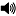
\includegraphics[width=0.3cm]{play.png} and \textbf{thite} 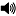
\includegraphics[width=0.3cm]{play.png} ?''); to facilitate mapping between visual and spoken word forms, the speaker button next to each word played the spoken word when clicked. In two catch trials, we asked participants to press the response button corresponding to the solution of a simple arithmetic problem. If participants learned the MN and PQ co-occurrence relationships \emph{and} used these relationships as a basis for similarity judgments, then we expected that participants would rate within-category pairs of words as more similar than cross-category pairs.

\begin{figure}[t]
  \begin{center}
    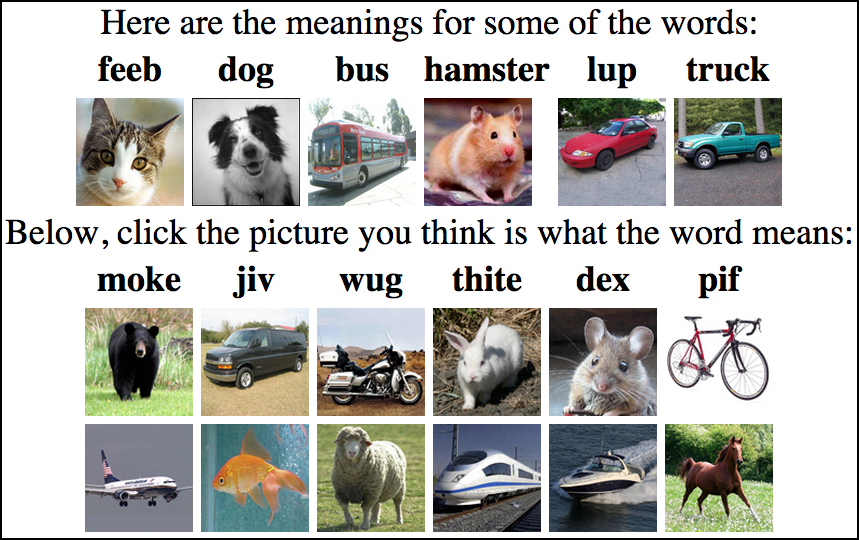
\includegraphics[width=8.5cm]{meaning-html-cropped.png}
    \caption{A screenshot of the referent assignment task.}
    \label{meaning-task}
  \end{center}
\end{figure}

\paragraph{Memory}
Participants listened to sentences and rated on a 5 point scale how confident they were that they had heard the sentence during exposure. We tested four types of sentences:

\begin{itemize}
\item \emph{Familiar} sentences heard during exposure.
\item \emph{Withheld} sentences not heard during exposure but conforming to the MNPQ structure.
\item \emph{Co-occurrence violation} sentences of the form MQ and PN.
\item \emph{Position violation} sentences of the form MM, NN, PP, and QQ.\footnote{ We only used position violation sentences that did not repeat the same word twice, e.g., we never presented $m_1 - m_1$.}
\end{itemize}

We presented sentences in random order such that there were no repeated words between consecutive trials. In two catch trials,\footnote{\label{catch-trials} In initial data collection, we did not include catch trials.  Let [A/3;B] denote the experimental condition with A/3 coherence and B exposures (e.g., [2/3;196] refers to the 2/3 coherence level with 196 exposures). In [0/3;196], 18 out of 40 participants did not receive catch trials. In [3/3;56], 30 out of 43 participants did not receive catch trials. In [3/3;126], 30 out of 40 participants did not receive catch trials. In [3/3;196], 30 out of 40 participants did not receive catch trials.} instead of a sentence from the MNPQ language, we played an audio instruction (which could not be repeated by participants) to press a specific response button.  If participants learned the MN and PQ co-occurrence relationships, then we expected that they would rate novel grammatical sentences as more familiar than the co-occurrence violation sentences.

\paragraph{Referent assignment}
We provided participants with referents for all of the Ms and Ps and asked them to choose referents for the Ns and Qs (Figure \ref{meaning-task}). At the top of the screen, we displayed the Ms and Ps in random order and we provided referents by displaying a single image underneath each word. The M and P referents were either animals (cat, dog, hamster) or vehicles (car, bus, truck); either Ms were animals and Ps were vehicles, or vice versa. Recall that some conditions contained \emph{familiar} M and P words; in these cases, we paired the known words with the obvious referents (e.g., ``dog'' was always paired with an image of a dog). Below the M and P words and their meanings, we displayed a row containing the N and Q words. Under each word, we displayed a two-alternative referent choice between an animal (the ``correct'' choice for N words) and vehicle words (the ``correct'' choice for Q words); participants made a choice by clicking on one of the two pictures. If participants learned the MN and PQ co-occurrence relationships \emph{and} and used them as a basis for inferences about word meaning, then we expected that referent assignment scores would reflect a tendency to choose similar referents for words in the same category. In addition, we hypothesized that, under these circumstances, participants would pick animals for Ns  and vehicles for Ps. This is because Ns consistently co-occurred with Ms, which we indicated referred to animals, and Qs consistently co-occurred with Ps, which we indicated referred to vehicles.

\subsection{Results and Discussion}
We excluded the 55 participants who did not correctly answer all of the catch trials.\footnote{ Recall that some participants -- mostly in the 3/3 conditions --  did not receive catch trials (see Footnote~\ref{catch-trials}). This does not bias the results in favor of our hypothesis; if anything, this weakens any effect of semantic coherence, as it introduces noise at the highest level of semantic coherence but not at any other level. Indeed, our results are not affected by including subjects who had catch trials and failed them.} We first present descriptive statistics of the memory task before analyzing the influence of coherence and exposure on distributional learning as measured by all three tasks. 

\begin{figure}[t]
  \begin{center}
    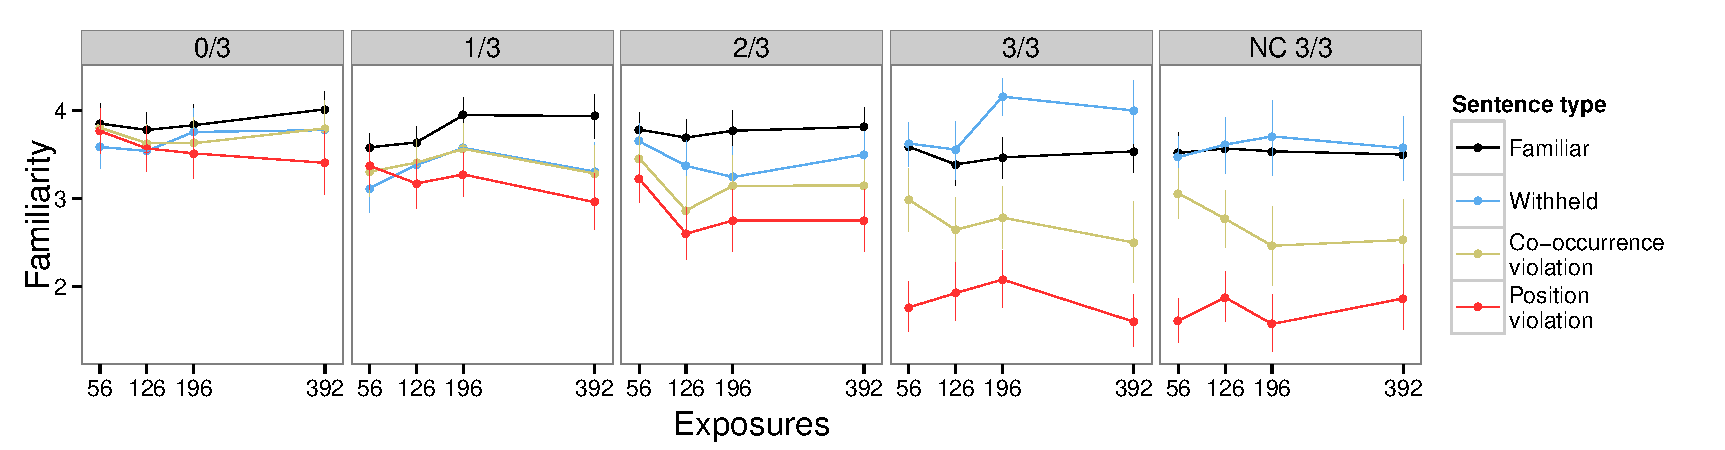
\includegraphics[width=1.0\linewidth]{x1-descriptive-memory} 
    \caption{Mean familiarity ratings for differente sentence types in Experiment 1.}
    \label{x1-descriptive-mem}
  \end{center}
\end{figure}

\subsubsection{Descriptive statistics for the memory task}

Figure~\ref{x1-descriptive-mem} shows mean familiarity ratings broken down by sentence type, coherence, and exposures. Within each coherence level, we looked for evidence of a familiarity ordering on sentence types. For each participant, we computed their mean familiarity rating for each sentence type. Then, at each coherence level, we ran 6 paired-sample t-tests comparing mean familiarity ratings across sentence types and corrected for multiple comparisons using the Holm procedure (Figure~\ref{familiarity-ordering-t-tests}). This yielded the following familiarity orderings:

0/3: F > W, P\\
1/3: F > W, C, P \, \, \, \textbf{\&} \, \, \, C > P\\
2/3: F > W > C > P\\
3/3: W > F > C > P\\

\noindent These familiarity orderings indicate that some learning occurred at every level of coherence. For example, participants at all levels of coherence rated familiar sentences as more familiar than position violation sentences. However, only participants at the 2/3 and 3/3 levels distinguished between withheld and co-occurrence violation sentences. This lends some support to the idea that positional regularities in MNPQ may be more influential than co-occurrence regularities.



\subsubsection{Effect of coherence and exposure}

For each dependent measure---memory, similarity, and referent assignment---we defined a within-participant score representing the sensitivity to the co-occurrence regularities in the language. We scaled all scores to lie in the interval [-1, 1], which allows for the following interpretation: scores below 0 indicate learning in the incorrect direction (e.g., preferring co-occurrence violation sentences over withheld sentences), while scores above 0 indicate learning in the correct direction.

The memory score measured the difference in familiarity ratings for withheld versus co-occurrence violation sentences. For each participant, we computed their memory score as the mean rating for withheld sentences (e.g., $m_1$--$n_1$) minus their mean rating for novel co-occurrence violation sentences (e.g., $m_1$--$q_1$). This difference had a minimum value of -4 and a maximum value of 4; we divided this difference by 4 to rescale it to lie in the interval [-1, 1]. Note that memory score did not include ratings for familiar or position-violation sentences.

The similarity score measured the difference between similarity ratings for within-category and cross-category pairs of words on the similarity task. For each participant, we computed their similarity score as their mean rating for within category pairs (e.g., $m_1$--$n_1$) minus their mean rating for cross category pairs (e.g., $m_1$--$q_1$). As with the memory scores, this yields a measure that lies in the interval [-4, 4], which we scaled to [-1, 1].

The referent assignment score measured the total number of correct choices in the referent assignment task. The lowest score was 0 and the highest possible score was 6. We rescaled this to the interval [-1, 1] by taking the raw number correct, subtracting 3, and then dividing by 3.

We analyzed the effects of coherence and exposure using linear models. First, we looked for main effects of coherence on score (i.e., the Condition coefficients in Table \ref{expt1-regressions}). Second, as we were interested in the relationship between amount of exposure and score, we looked for exposure $\times$ coherence interactions. A significant interaction (e.g., the E $\times$ C coefficients in Table \ref{expt1-regressions}) would indicate a difference in how \emph{efficiently} the statistical learning process makes use of evidence at different coherence levels. For all scores, we coded coherence as a categorical variable and analyzed the data using a regression which modeled the mean score in a participant group (e.g., 3/3-56) as an interactive function of the number of exposures (e.g., 56) times the condition (e.g., full coherence). In other words, our regression equation was score $\sim$ exposures $\times$ condition. Results are shown in Figure \ref{expt1-results}.

To examine the differences between the different coherence levels, we used Helmert contrasts analyzing (i) the difference between the 1/3 and 0/3 conditions, (ii) the difference between the 2/3 condition and the 0/3 and 1/3 conditions combined, and (iii) the difference between the 3/3 condition and the 0/3, 1/3, and 2/3 conditions combined. Results of these analyses are shown in Table \ref{expt1-regressions}. Before detailing the results for each measure, we will first state the two broad patterns of results. First, learning was highest in 3/3 condition. Second, we found the strongest evidence of statistical efficiency (i.e., sensitivity to the amount of exposure) in the 3/3 condition.

\begin{figure}[t]
  \begin{center}
    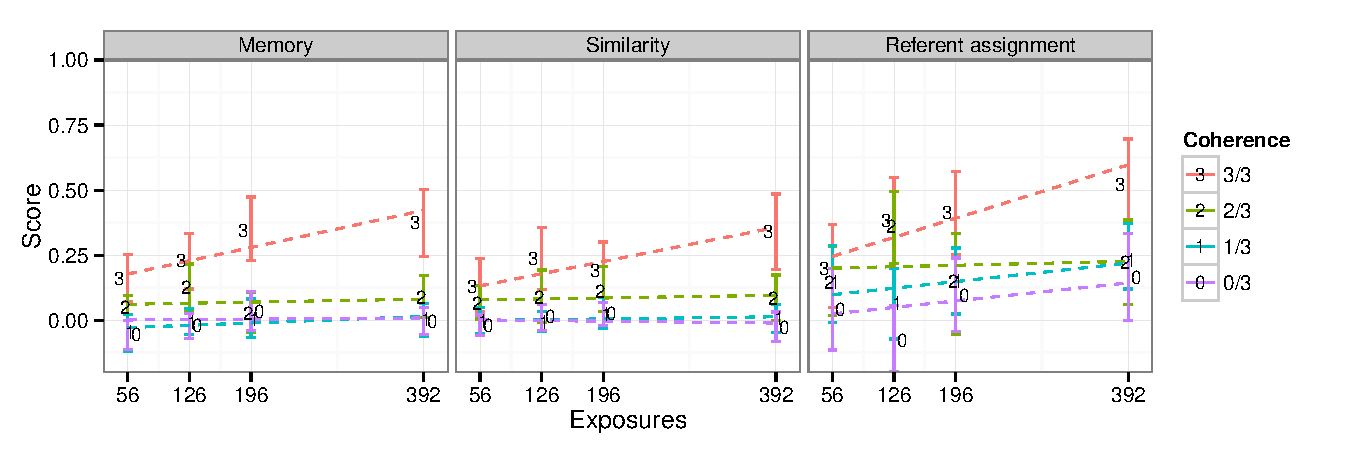
\includegraphics[width=1.0\linewidth]{x1}
    \caption{Experiment 1 results. Each plot shows data for one measure (memory, similarity, referent assignment) in Experiment 1. Scores ranged from -1 to 1. Data points show condition means, error bars show 95\% CIs, and dashed lines show the best-fitting linear regression.}
    \label{expt1-results}
  \end{center}
\end{figure}

\newcommand{\ww}{\color{white}{*}} \newcommand\T{\rule{0pt}{2.1ex}}

\begin{table}[ht]
  \caption{Regression model for Experiment 1. For readability, exposure values were divided by 1000.}
  \label{expt1-regressions} 
  \begin{center}
  \footnotesize{
    \begin{tabular}{l r r r r}
      \hline
      Regressor & $\beta$ & Std Error & $t$ & $p$ \\ \hline
      \multicolumn{5}{l}{\T \textbf{Memory}: $R^2$ = 0.18, $F$(7, 615) = 20.01 \T}\\ 
      Intercept &  0.0359 &  0.018 &  1.91 & 0.056\ww\\
      Condition: 1/3 -- (0/3) & -0.0005 &  0.027 & -0.01 & 0.984\ww\\
      Condition: 2/3 -- (0/3,1/3) &  0.0309 &  0.014 &  2.09 & <0.05*\\
      Condition: 3/3 -- (0/3,1/3,2/3) &  0.0396 &  0.010 &  3.65 & <0.001*\\
      Exposures &  0.2346 &  0.083 &  2.81 & <0.005*\\
      E $\times$ C: 1/3 -- (0/3) &  0.0033 &  0.120 &  0.02 & 0.977\ww\\
      E $\times$ C: 2/3 -- (0/3,1/3) & -0.0215 &  0.065 & -0.32 & 0.743\ww\\
      E $\times$ C: 3/3 -- (0/3,1/3,2/3) &  0.1326 &  0.048 &  2.73 & <0.01* \\
      \hline

      \multicolumn{5}{l}{\T \textbf{Similarity}: $R^2$ = 0.12, $F$(7, 615) = 12.09 \T}\\
      Intercept &  0.0501 &  0.018 &  2.64 & <0.01*\\
      Condition: 1/3 -- (0/3) & -0.0070 &  0.027 & -0.25 & 0.798\ww\\
      Condition: 2/3 -- (0/3,1/3) &  0.0237 &  0.014 &  1.59 & 0.112\ww\\
      Condition: 3/3 -- (0/3,1/3,2/3) &  0.0224 &  0.010 &  2.04 & <0.05*\\
      Exposures &  0.1487 &  0.084 &  1.77 & 0.077\ww\\
      E $\times$ C: 1/3 -- (0/3) &  0.0514 &  0.121 &  0.42 & 0.671\ww\\
      E $\times$ C: 2/3 -- (0/3,1/3) &  0.0208 &  0.066 &  0.31 & 0.754\ww\\
      E $\times$ C: 3/3 -- (0/3,1/3,2/3) &  0.1373 &  0.048 &  2.80 & <0.01* \\
      \hline

      \multicolumn{5}{l}{\T \textbf{Referent assignment}:  $R^2$ = 0.06, $F$(7, 611) = 6.45 \T}\\
      Intercept &  0.1087 &  0.036 &  3.01 & <0.005*\\
      Condition: 1/3 -- (0/3) &  0.0664 &  0.052 &  1.26 & 0.208\ww\\
      Condition: 2/3 -- (0/3,1/3) &  0.0616 &  0.028 &  2.17 & <0.05*\\
      Condition: 3/3 -- (0/3,1/3,2/3) &  0.0359 &  0.020 &  1.72 & 0.084\ww\\
      Exposures &  0.4577 &  0.159 &  2.86 & <0.005*\\
      E $\times$ C: 1/3 -- (0/3) & -0.0919 &  0.230 & -0.39 & 0.690\ww\\
      E $\times$ C: 2/3 -- (0/3,1/3) & -0.1257 &  0.126 & -0.99 & 0.319\ww\\
      E $\times$ C: 3/3 -- (0/3,1/3,2/3) &  0.1292 &  0.093 &  1.38 & 0.167\ww \\
      \hline
    \end{tabular}
  }
  \end{center}
\end{table}

\subsubsection{Task results}

We report performance on each of the three tasks separately.

\paragraph{Memory} More exposure led to higher memory scores, as there was a main effect of exposure. Higher coherence also led to higher memory scores; 2/3 scores were significantly higher than scores from the 0/3 and 1/3 conditions combined and 3/3 scores were significantly higher than scores from the rest of the conditions combined. Because 2/3 and 3/3 scores both outperformed all the respective lower levels of coherence, we also computed this model using coherence as a continuous variable; the continuous coherence regressor significantly predicted increases in score, $\beta = 0.06$, $t(619) = 3.86$, $p < 0.0005$, suggesting that parametrically increasing coherence results in parametric increases in memory score.

% condition.num 6.730e-02 1.743e-02 3.862 0.000124 ***

Additionally, the effect of exposures on memory score was significantly higher in 3/3 than in the other conditions combined (i.e., there was a significant exposure $\times$ coherence interaction), suggesting greater efficiency of statistical learning in 3/3. Thus, more semantically coherent linguistic input (1) bolstered memory for the MN and PQ co-occurrence regularities and (2) increased the efficiency of the statistical learning process responsible for learning those regularities, at least in the 3/3 condition.

\paragraph{Similarity} Similarity scores were higher in the 3/3 condition than the other conditions combined. In addition, the effect of exposures on score was significantly higher in the 3/3 condition than in the other conditions combined, as there was a significant exposure $\times$ coherence interaction. Thus, more coherent linguistic input (1) increased the distinction between within-category and cross-category pairs of words and (2) increased the efficiency of the statistical learning of such distinctions, at least in the 3/3 condition.

\paragraph{Referent assignment}

2/3 scores were significantly higher than 0/3 and 1/3 scores combined. 3/3 scores were marginally higher than the rest of the scores combined, possibly because 3/3 coherence and 2/3 coherence may confer comparable advantages on this task. We also computed this model using coherence as a continuous variable; the continuous coherence regressor significantly predicted increases in score, $\beta = 0.09$, $t(619) = 2.87$, $p < 0.005$, suggesting that \emph{parametrically} increasing coherence results in \emph{parametric} increases in referent assignment score. None of the interaction terms reached significance, indicating that the amount of exposure to the language and greater coherence independently increased the ability to assign N and Q words to the correct referents.

% parametric increase stuff: condition.num 9.434e-02 3.285e-02 2.872 0.00422 **

\subsubsection{Summary}

In Experiment 1, we found that semantic coherence (1) increased ability to distinguish novel grammatical sentences from sentences violating co-occurrence regularities in the memory task, (2) sharpened sensitivity to category boundaries based on the co-occurrence regularities in the similarity task, and (3) increased inductive bias in associating target words with referents.

The context words that participants heard in Experiment 1 included words with familiar meanings that were organized into coherent categories. Would it be enough to merely have familiar words without coherence or the reverse? How does the effect of semantic coherence depend on each? In Experiment 2 we test for the effect of familiar meaning and in Experiment 3, we test for the effect of coherence. In Experiment 2, we remove familiar meaning by exposing learners to languages with phonological, as opposed to semantic, coherence. In Experiment 3, we remove coherence by exposing learners to languages with context words that are familiar but do not adhere to any obvious semantic organization.

\section{Experiment 2: Phonological coherence}

In Experiment 2, we investigated whether learners could learn the language used in  Experiment 1 when the context words (Ms and Ps) exhibited phonological, rather than semantic, coherence. It is worth emphasizing that we manipulated phonological coherence in the \emph{context} words, whereas previous work has manipulated phonological coherence of the \emph{target} words. Previous work has shown that learning is facilitated when target words have both distributional and phonological regularities. By contrast, we are interested in how distributional learning for one category of words varies as a function of \emph{other} words in the linguistic environment.

We tested three types of coherence: onset, rime, and syllable count. We selected these kinds of coherence because work in other areas suggests that these kinds of coherence may reliably occur in natural language or facilitate distributional learning when applied to \emph{target} words. Onset coherence might facilitate learning due to sound symbolism (e.g., words that start with \emph{gl} have similar meanings: glimmer, glow, gleam). Rime coherence can occur in languages that require gender-marking agreement between nouns and verbs. Finally, syllable count coherence has been shown to facilitate learning when applied to target words \citep{lany2010}. Thus, we investigated it to determine whether it also facilitates learning when applied to context words.

\subsection{Method}
\subsubsection{Participants} 
530 MTurk workers, recruited as in Experiment 1, participated in the study.

\subsubsection{Materials}
The three types of phonological coherence\footnote{\label{change-of-stimuli} The stimuli for the rime and syllable count conditions differ from those in the rest of our conditions. For the rest of the conditions, we used a text-to-speech web service provided by Google to generate the audio stimuli (see Footnote \ref{tts}) for the bulk of the conditions. However, the available voices on this service changed during our experiment. Thus, we generated new stimuli for the rime and syllable count conditions using commercially available software, NaturalReader 10. To ensure that the old and new stimuli were comparable, we performed a partial replication of Experiment 1 using the new synthesis engine; the difference old and new stimuli did not appear to make a substantial difference. See Appendix \ref{old-vs-new} for comparisons.} were:

\begin{itemize}
\item \emph{Onset}. Ms all started with one consonant cluster (pladge, plaaf, plab) and Ps all started with another (zof, zawd, zawsh).
\item \emph{Rime}. Ms all ended with one vowel (calo, pawmo, marfo) and Ps all ended with another (zaygee, kaisee, tetchee).
\item \emph{Syllable count}. Ms were disyllabic (coomo, fengle, kaisee) and Ps were monosyllabic (gope, jic, skeege).
\end{itemize}

\subsubsection{Design and Procedure}
The method was identical to that of Experiment 1.

\subsection{Results and Discussion}

We discarded the 42 participants who did not pass all the catch trials. Results are graphed in Figure \ref{expt23-results}.

\subsubsection{Descriptive statistics for the memory task}

\begin{figure}[t]
  \begin{center}
    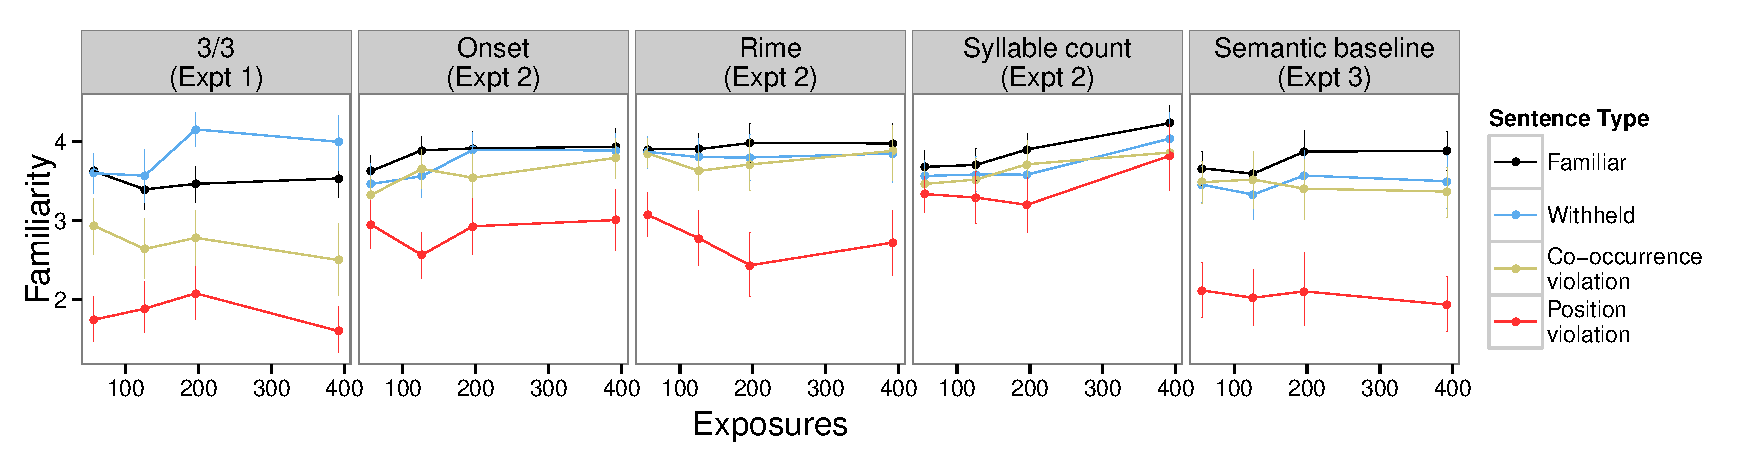
\includegraphics[width=1.0\linewidth]{x23-descriptive-memory}
    \caption{Mean familiarity ratings for different sentence types in Experiments 2 and 3. For comparison, we also include the 3/3 coherence condition from Experiment 1.}
    \label{x23-descriptive-mem}
  \end{center}
\end{figure}

Figure~\ref{x23-descriptive-mem} shows mean familiarity ratings broken down by sentence type, coherence, and exposures. As in the analyses for Experiment 1, we computed a familiarity ordering on sentence types within each phonological coherence condition using paired sample t-tests (Figure~\ref{familiarity-ordering-t-tests}):

\begin{tabular}{l l}
Onset: & F > W > C > P\\
Rime: & F > W $\approx$ C > P\\
Syllable count: & F > W $\approx$ C > P\\
\end{tabular}\vskip 0.5em


% condition       mean        sd
% 1     phn3b 0.03311258 0.1786535
% 2      sem2 0.06893939 0.2384553
% 3      sem3 0.27246732 0.3607215

% Two Sample t-test

% data:  s(agg, condition == "phn3b")$mem.score and s(agg, condition == "sem2")$mem.score
% t = -1.5006, df = 314, p-value = 0.1345
% alternative hypothesis: true difference in means is not equal to 0
% 95 percent confidence interval:
% -0.08280317  0.01114955
% sample estimates:
% mean of x  mean of y 
% 0.03311258 0.06893939 


% Two Sample t-test

% data:  s(agg, condition == "phn3b")$mem.score and s(agg, condition == "sem3")$mem.score
% t = -7.3161, df = 302, p-value = 2.316e-12
% alternative hypothesis: true difference in means is not equal to 0
% 95 percent confidence interval:
% -0.3037356 -0.1749739
% sample estimates:
% mean of x  mean of y 
% 0.03311258 0.27246732


\noindent Thus, participants in the rime and syllable count conditions distinguished between all types of sentences except for withheld and co-occurrence violation sentences, indicating some learning of the language but not of the co-occurrence regularities. By contrast, participants in the onset condition did appear to learn the co-occurrence regularities, rating withheld sentences as significantly more familiar than co-occurrence violation sentences. The ordering for onset phonological coherence is the same as the ordering for 2/3 semantic coherence. To understand the degree of co-occurrence structure learning for the onset condition, we compared onset memory scores with 2/3 and 3/3 memory scores. Onset scores (M = 0.03, SD = 0.17) were not significantly different from 2/3 scores (M = 0.06, SD = 0.23), $t$(314) = -1.5, $p$ = 0.13, but they were significantly lower than 3/3 scores (M = 0.27, SD = 0.36), $t$(302) = -7.31, $p$ < 0.001.

\subsubsection{Effects of condition and exposure}

\begin{figure}[t]
  \begin{center}
    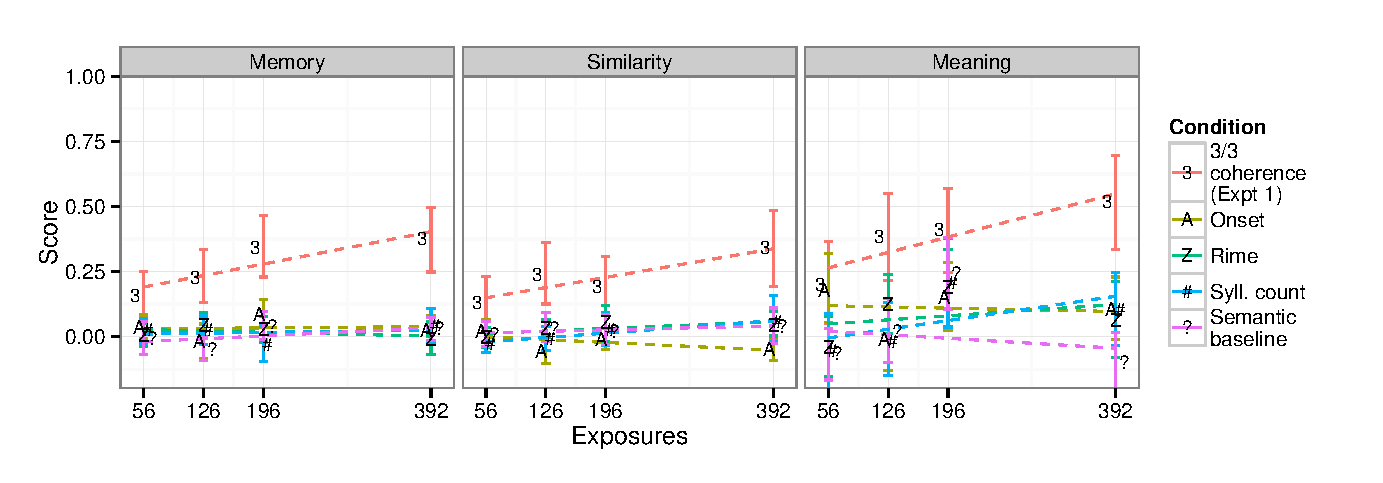
\includegraphics[width=1.0\linewidth]{x23}
    \caption{Experiments 2 and 3 results. Each plot shows data for one measure (memory, similarity, referent assignment). Scores ranged from -1 to 1. Points show condition means, error bars show 95\% CIs, and dashed lines show the best-fitting linear trend. For comparison, we also include the 3/3 coherence condition from Experiment 1.}
    \label{expt23-results}
  \end{center}
\end{figure}

\begin{table}[t]
  \caption{Regression model for Experiments 2 and 3. For readability, exposure values were divided by 1000.}
  \label{expt23-regression}
  \begin{center} 
    \scriptsize{
      \begin{tabular}{l r r r r}
        \hline
        Predictor & $\beta$ & Std Error & $t$ & $p$ \\ \hline
        \multicolumn{5}{l}{\T \textbf{Memory}: $R^2$ = 0.009, $F$(7, 631) = 0.88 \T}\\
        Intercept & -0.0341 &  0.027 & -1.24 & 0.215\ww\\
        Condition: Onset -- 0/3 &  0.0626 &  0.038 &  1.64 & 0.100\ww\\
        Condition: Rime -- 0/3 &  0.0652 &  0.035 &  1.82 & 0.068\ww\\
        Condition: Syllable count -- 0/3 &  0.0410 &  0.038 &  1.06 & 0.287\ww\\
        Condition: Semantic incoherent -- 0/3 &  0.0055 &  0.038 &  0.14 & 0.883\ww\\
        Exposures &  0.1201 &  0.119 &  1.00 & 0.316\ww\\
        E $\times$ C: Onset -- 0/3 & -0.0948 &  0.170 & -0.55 & 0.577\ww\\
        E $\times$ C: Rime -- 0/3 & -0.1950 &  0.161 & -1.20 & 0.228\ww\\
        E $\times$ C: Syllable count -- 0/3 & -0.0735 &  0.167 & -0.43 & 0.660\ww\\
        E $\times$ C: Semantic incoherent -- 0/3 &  0.0388 &  0.162 &  0.23 & 0.811\ww \\
        \hline

        \multicolumn{5}{l}{\T \textbf{Similarity}: $R^2$ = 0.02, $F$(7, 631) = 2.51 \T}\\
        Intercept &  0.0110 &  0.025 &  0.43 & 0.662\ww\\
        Condition: Onset -- 0/3 & -0.0031 &  0.035 & -0.08 & 0.928\ww\\
        Condition: Rime -- 0/3 & -0.0064 &  0.033 & -0.19 & 0.846\ww\\
        Condition: Syllable count -- 0/3 & -0.0455 &  0.035 & -1.27 & 0.201\ww\\
        Condition: Semantic incoherent -- 0/3 & -0.0007 &  0.035 & -0.02 & 0.982\ww\\
        Exposures & -0.0607 &  0.110 & -0.54 & 0.582\ww\\
        E $\times$ C: Onset -- 0/3 & -0.0937 &  0.157 & -0.59 & 0.550\ww\\
        E $\times$ C: Rime -- 0/3 &  0.1951 &  0.149 &  1.30 & 0.191\ww\\
        E $\times$ C: Syllable count -- 0/3 &  0.3049 &  0.154 &  1.97 & <0.05*\\
        E $\times$ C: Semantic incoherent -- 0/3 &  0.1401 &  0.150 &  0.93 & 0.350\ww \\
        \hline

        \multicolumn{5}{l}{\T \textbf{Referent assignment}: $R^2$ = 0.01, $F$(7, 629) = 1.12 \T}\\
        Intercept & -0.0553 &  0.068 & -0.81 & 0.418\ww\\
        Condition: Onset -- 0/3 &  0.1776 &  0.094 &  1.88 & 0.060\ww\\
        Condition: Rime -- 0/3 &  0.0916 &  0.088 &  1.03 & 0.301\ww\\
        Condition: Syllable count -- 0/3 &  0.0234 &  0.095 &  0.24 & 0.806\ww\\
        Condition: Semantic incoherent -- 0/3 &  0.0868 &  0.094 &  0.91 & 0.359\ww\\
        Exposures &  0.5462 &  0.296 &  1.84 & 0.066\ww\\
        E $\times$ C: Onset -- 0/3 & -0.6122 &  0.421 & -1.45 & 0.146\ww\\
        E $\times$ C: Rime -- 0/3 & -0.3243 &  0.400 & -0.80 & 0.418\ww\\
        E $\times$ C: Syllable count -- 0/3 & -0.0692 &  0.414 & -0.16 & 0.867\ww\\
        E $\times$ C: Semantic incoherent -- 0/3 & -0.7403 &  0.402 & -1.83 & 0.066\ww \\
        \hline
      \end{tabular}
    }
  \end{center}
\end{table}

Using a regression model with main effects of exposure and condition and an exposure $\times$ condition interaction, we compared each phonological condition with the 0/3 condition of Experiment 1 using a regression model (Table \ref{expt23-regression}).

\paragraph{Memory} 
There was no effect of exposure or condition---none of the phonological condition scores were significantly different from 0/3 scores. None of the exposure by condition interaction terms were significant.

\paragraph{Similarity}
Again, we found no main effect of exposure or condition. One interaction term was significant: there appeared to be greater efficiency of statistical learning in the syllable count condition than in the 0/3 condition.

\paragraph{Referent assignment}
Again, we found no main effect of exposure or condition. None of the exposure by condition interaction terms were significant.

In sum, with one exception, participants in all three phonological conditions appeared not to have acquired separate N and Q categories; phonological coherence was virtually indistinguishable from 0/3 coherence in terms of facilitating MNPQ learning. The one exception is that participants in the onset coherence condition were able to distinguish withheld from co-occurrence violation sentences, matching 2/3 participants' performance in this regard. However, unlike 2/3 coherence, onset coherence did not appear to confer benefits in the similarity or referent assignment tasks. Thus, this broad pattern of results suggests that the mere presence of \emph{some} kind of coherence in the context words is not what drives the effects of semantic coherence. In Experiment 3, we consider whether the mere presence of familiar words (semantic baseline) aids MNPQ learning.

\section{Experiment 3: Semantic baseline}

In Experiment 1, Ms and Ps were all familiar words obeying a taxonomic organization. In Experiment 3, we explored a language with familiar words but no semantic organization---that is, whether a semantic baseline language facilitates distributional learning. We might expect this baseline condition to facilitate learning due to lower memory demands---known words tax the memory system less, which might free learners to identify co-occurrence regularities.

\subsection{Methods}
\subsubsection{Participants}
162 MTurk workers, recruited as in Experiment 1. Note that there were many fewer participants in Experiment 3 because there was only one condition, compared to four conditions in Experiment 1 and three conditions in Experiment 2.

\subsubsection{Materials}
In the semantic baseline language, the specific M and P words were drawn randomly for each participant from the pool \{\emph{shelf}, \emph{glove}, \emph{rain}, \emph{leash}, \emph{card}, \emph{ball}\}. In the referent assignment task, these known words were paired with images of the obvious referents (e.g., \emph{card} with a picture of a card). Compared to the context words in Experiment 1, these words are fairly well matched in frequency (see \ref{word-freqs}).

\begin{table}
  \begin{center}
  \caption{Context word frequencies from Experiments 1 and 3 sorted by decreasing frequency. Frequencies were retrieved from Google N-grams data for the year 1999.}
  \label{word-freqs}
  \footnotesize{
    \begin{tabular}{l l l}
      Word &  Frequency (\%) & Experiment\\
      \hline
      Car & 0.0091 & 1\\
      Dog & 0.0042 & 1\\
      Card & 0.0035 & 3\\
      Ball & 0.0035 & 3\\
      Rain & 0.0030 & 3\\
      Bus & 0.0026 & 1\\
      Cat & 0.0021 & 1\\
      Truck & 0.0017 & 1\\
      Shelf & 0.00094 & 3\\
      Glove & 0.00029 & 3\\
      Leash & 0.00015 & 3\\
      Hamster & 0.000099 & 1\\
      \hline
    \end{tabular}}
  \end{center}
\end{table}

\subsubsection{Design and procedure}
The method was identical to that of Experiment 1.

\subsection{Results and Discussion}
We discarded the 18 participants who did not pass all the catch trials. 


\subsubsection{Descriptive statistics of the memory task}
As in Experiment 1, we computed an ordering on the sentence types in the memory task: F > W $\approx$ C > P. This indicates that participants were able to learn some regularities in the language, but not the co-occurrence regularities.

\subsubsection{Effect of exposure}

Results are graphed in Figure \ref{expt23-results}. See Table \ref{expt23-regression} for regression results.

\paragraph{Memory}
Baseline scores were not significantly different from 0/3 scores and baseline efficiency was not significantly different from 0/3 efficiency.

\paragraph{Similarity}
Baseline scores were not significantly different from 0/3 scores and baseline efficiency was not significantly different from 0/3 efficiency.

\paragraph{Referent assignment}
Baseline scores were not significantly different from 0/3 scores and baseline efficiency was not significantly different from 0/3 efficiency.\\

Apparently, the baseline input appeared to have provided no benefit compared to the novel words of the 0/3 condition, suggesting that the presence of known words by itself does not aid MNPQ learning.

\section{General Discussion}
Can people learn about words from co-occurrence statistics? Previous work on distributional learning based on co-occurrence presented a paradox: While computational models suggest that distributional statistics are a powerful source of information, experiments with humans show consistent failures. Our experiments suggest a partial resolution. For people, distributional learning is facilitated by semantic coherence: Knowing that Alice associated with X and Y tells us something about Alice only if X and Y are already meaningful and meaningfully related to one another. Removing either the meanings of the individuals or the coherence of the relationship between them (cf. ``word salad'') removes the facilitation. 

What is the mechanism by which semantic coherence facilitates learning? Perhaps learners use semantic coherence to infer the topic of discourse and then tag novel words with these topics. For example, in the highest semantic coherence condition of our experiments, participants may have learned that the topic of discourse is either animal-related or vehicle-related and then tracked co-occurrence between these topics and novel words \citep{frank2013}. Such a proposal is congruent with the ``preferential acquisition'' idea of Hills and colleagues \citeyearpar{hills2009, hills2010}, in which the easiest words to learn are those that connect well with others in the learning environment. 

Our finding that phonological coherence does not facilitate learning may at first appear at odds with experiments that have reached the opposite conclusion \citep{frigo1998, lany2010, monaghan2005}. But previous work has applied phonological regularities to the target words (the words that experimenters measure learning for).  In contrast, in order to permit comparison with the semantic coherence conditions, we applied the regularities to the context words (the words that co-occurred with the target words). In other words, previous experiments used target coherence, while we used context coherence. In our experiment, the target categories themselves did not have phonological regularity but they reliably co-occurred with context categories that did. We speculate that this subtle but substantial difference explains the different patterns we observed.

\subsection{Limitations and Future Directions}

The limitations of our approach may serve as inspiration for future work. First, we explored a single artificial language, MNPQ, because past research has shown that it is largely resistant to distributional learning. While less is known about other languages, \cite{reeder2009} found successful distributional learning for the (Q)AXB(R) language, which fixes a positional confound in MNPQ (Ms and Ps are always sentence-initial and Ns and Qs are always sentence-final), suggesting that learning is sensitive to the language structure. How do variations across language structure interact with factors like semantic and phonological coherence? 

Second, we investigated a single type of semantic coherence, where context words fell into two different taxonomic categories, and a single syntactico-semantic construction that biases interpretation towards concrete nouns (e.g., ``cat and wug''). These choices likely affected the magnitude of the effects we observed. While the simplicity and transparency of our semantic categories likely facilitated learning, our use of concrete noun targets might even have understated the effects of coherence. Distributional learning through semantic coherence might be especially useful for words like verbs and adjectives \citep{redington1998}, where referential grounding provides less information about meaning \citep{gleitman1990}.

Finally, while our study addressed one shortcoming of much artificial language research---the lack of semantic grounding---it is still congruent with other artificial language research in scale (6 words in a single exposure session). Small-scale experiments do not allow strong inferences about the importance of different factors in lexical learning \citep{romberg2010, frank2013}. A mixture of computational analyses and larger-scale experiments are necessary to understand the role semantic coherence---and distributional learning more generally---plays in language learning.

\subsection{Conclusion}
Since Firth's edict that we shall know a word ``by the company it keeps,'' two lines of research have yielded apparently conflicting results. Although computational models suggest that distributional information is a powerful information source, artificial language learning experiments have suggested a more dubious outlook. Our results here may help to close this gap between the experimental and the computational. On the basis of our findings, we suggest a small modification to Firth's maxim: You shall know a word \emph{if you know} the company it keeps.

\newpage
\bibliographystyle{apacite}
\bibliography{references}

\appendix
\section{Old versus new stimuli comparison}
\label{old-vs-new}

We performed a partial replication of Experiment 1 with the new stimuli. We collected data in four out of the sixteen experimental conditions and the results mirror those found with the old stimuli:

\begin{center}
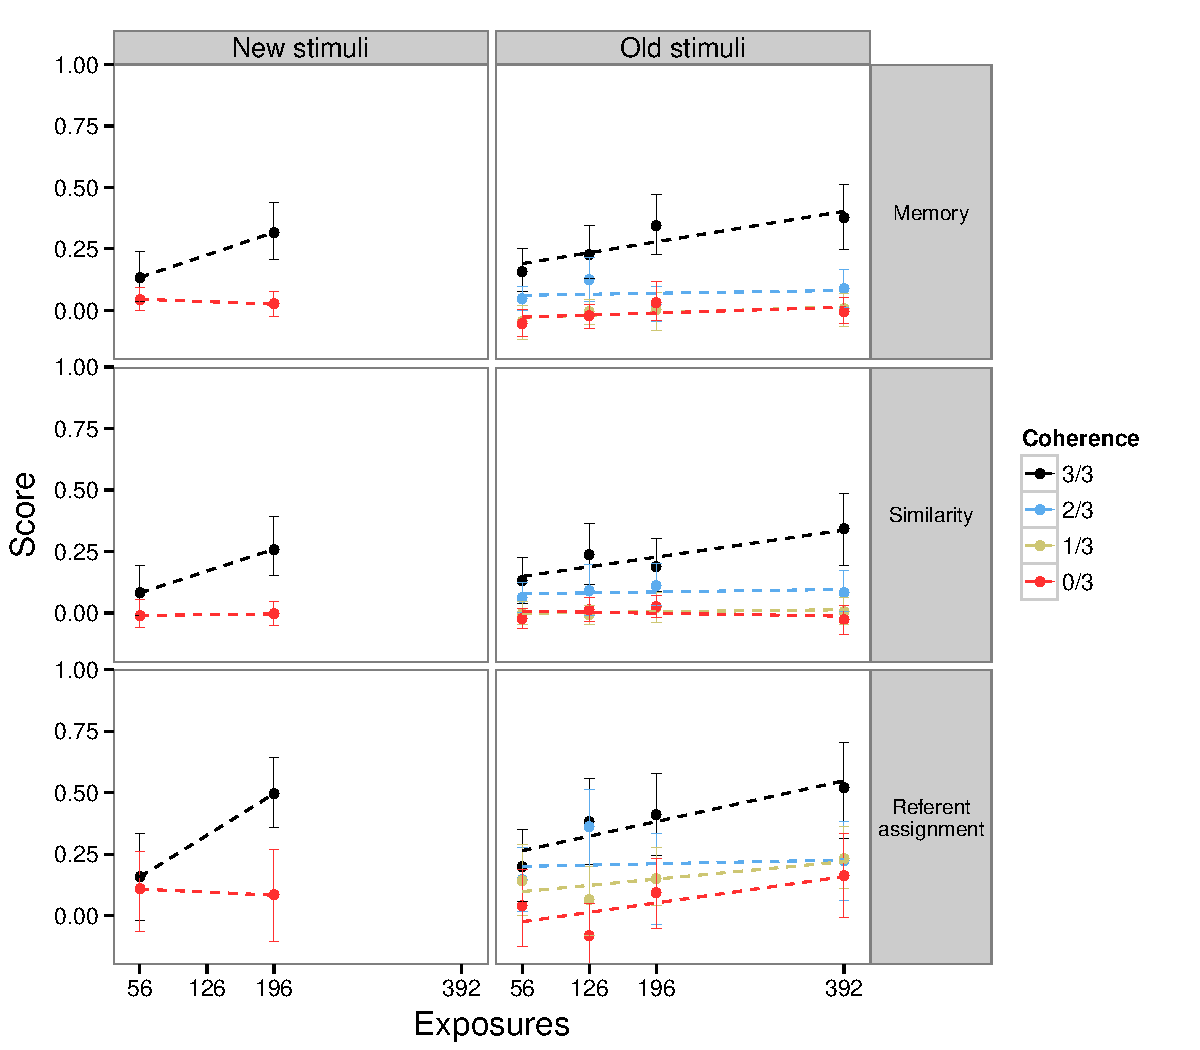
\includegraphics[width=0.9\linewidth]{stim-comparison} \\

\end{center}


\appendix
\section{$t$-tests for familiarity orderings in the memory task}

\begin{figure}[h]
  \begin{center}
    \begin{tabular}{ c c}

      \textbf{0/3 coherence}: df = 150 & \textbf{1/3 coherence}: df = 153\\
      
      {
        % -------------- none --------------
        % df = 150 

        % Pairwise comparisons using paired t tests 

        % data:  e$mem.score and e$type 

        %          familiar withheld cross  
        % withheld 0.01266  -        -      
        % cross    0.06278  0.48454  -      
        % position 0.00029  0.21723  0.08529

        % P value adjustment method: holm 
        \small

        \begin{tabular}{| l | l |  l | l |}
          \hline
          & F              & W           & C \\ 
          \hline
          W & $p$ = 0.01*  &             &\\
          \hline
          C & $p$ = 0.06 &  $p$ = 0.48 & \\
          \hline
          P & $p$ < 0.001* &  $p$ = 0.21 &  $p$ = 0.08 \\
          \hline
        \end{tabular}
      } & 

      {
        % -------------- sem1 --------------
        % df = 153 

        % Pairwise comparisons using paired t tests 

        % data:  e$mem.score and e$type 

        %          familiar withheld cross
        % withheld 7.4e-08  -        -    
        % cross    3.8e-06  0.525    -    
        % position 2.1e-12  0.085    0.018

        \small
        \begin{tabular}{| l | l |  l | l |}
          \hline
          & F               & W           & C \\ 
          \hline
          W &  $p$ < 0.001* &             &\\
          \hline
          C &  $p$ < 0.001* &  $p$ = 0.52 &\\
          \hline
          P &  $p$ < 0.001* &  $p$ = 0.08 &  $p$ = 0.01*\\
          \hline
        \end{tabular}
      }\\

      \textbf{2/3 coherence}: df = 164 & \textbf{3/3 coherence}: df = 152\\

      {

        % -------------- sem2 --------------
        % df = 164 

        % Pairwise comparisons using paired t tests 

        % data:  e$mem.score and e$type 

        %          familiar withheld cross  
        % withheld 1.2e-05  -        -      
        % cross    4.0e-14  0.00056  -      
        % position < 2e-16  3.5e-11  0.00056

        % P value adjustment method: holm 


        \small
        \begin{tabular}{| l | l |  l | l |}
          \hline
          & F                           & W                         & C \\ 
          \hline
          W &  $p$ < 0.001*  &                           &\\
          \hline
          C &  $p$ < 0.001*  &  $p$ < 0.001*  &\\
          \hline
          P &  $p$ < 0.001* &  $p$ < 0.001*  &  $p$ < 0.001*\\
          \hline
        \end{tabular}
      } & 

      {

        % -------------- sem3 --------------
        % df = 152 

        % Pairwise comparisons using paired t tests 

        % data:  e$mem.score and e$type 

        % familiar withheld cross  
        % withheld 0.00016  -        -      
        % cross    4.4e-16  4.4e-16  -      
        % position < 2e-16  < 2e-16  4.4e-16

        % P value adjustment method: holm 

        \small
        \begin{tabular}{| l | l |  l | l |}
          \hline
          & F                            & W                         & C \\ 
          \hline
          W &  $p$ < 0.001*  &                           &\\
          \hline
          C &  $p$ < 0.001*  &  $p$ < 0.001*   &\\
          \hline
          P &  $p$ < 0.001* &  $p$ < 0.001*  &  $p$ < 0.001*\\
          \hline
        \end{tabular}
      }\\

      \textbf{Onset}: df = 150 & \textbf{Rime}: df = 187\\

      % -------------- onset --------------
      % Pairwise comparisons using paired t tests 

      % data:  e$mem.score and e$type 

      % familiar withheld cross
      % withheld 0.04833  -        -    
      % cross    0.00012  0.04833  -    
      % position < 2e-16  < 2e-16  6e-15

      % P value adjustment method: holm 
      {
        \small

        \begin{tabular}{| l | l |  l | l |}
          \hline
          & F              & W           & C \\ 
          \hline
          W & $p$ = 0.04*  &             &\\
          \hline
          C & $p$ < 0.001* &  $p$ = 0.04* & \\
          \hline
          P & $p$ < 0.001* &  $p$ < 0.001* &  $p$ < 0.001* \\
          \hline
        \end{tabular}
      } & 

      % -------------- rime --------------
      % Pairwise comparisons using paired t tests 

      % data:  e$mem.score and e$type 

      % familiar withheld cross 
      % withheld 0.0969   -        -     
      % cross    0.0021   0.1526   -     
      % position <2e-16   <2e-16   <2e-16

      % P value adjustment method: holm 
      {
        \small
        \begin{tabular}{| l | l |  l | l |}
          \hline
          & F               & W           & C \\ 
          \hline
          W &  $p$ = 0.09 &             &\\
          \hline
          C &  $p$ = 0.002* &  $p$ = 0.15 &\\
          \hline
          P &  $p$ < 0.001* &  $p$ < 0.001* &  $p$ < 0.001*\\
          \hline
        \end{tabular}
      }\\

      \textbf{Syllable count}: df = 148 & \textbf{Semantic baseline}: df = 143 \\

      % -------------- syll.count --------------
      % Pairwise comparisons using paired t tests 

      % data:  e$mem.score and e$type 

      % familiar withheld cross  
      % withheld 0.00623  -        -      
      % cross    0.00011  0.30439  -      
      % position 4.5e-08  0.00152  0.01645

      % P value adjustment method: holm 
      {
        \small
        \begin{tabular}{| l | l |  l | l |}
          \hline
          & F                           & W                         & C \\ 
          \hline
          W &  $p$ < 0.006*  &                           &\\
          \hline
          C &  $p$ < 0.001*  &  $p$ = 0.30  &\\
          \hline
          P &  $p$ < 0.001* &  $p$ = 0.001*  &  $p$ = 0.01*\\
          \hline
        \end{tabular}
      } & 

      % -------------- baseline --------------
      % Pairwise comparisons using paired t tests 

      % data:  e$mem.score and e$type 

      % familiar withheld cross  
      % withheld 6.8e-05  -        -      
      % cross    6.8e-05  0.83     -      
      % position < 2e-16  < 2e-16  < 2e-16

      % P value adjustment method: holm 
      {
        \small
        \begin{tabular}{| l | l |  l | l |}
          \hline
          & F                            & W                         & C \\ 
          \hline
          W &  $p$ < 0.001*  &                           &\\
          \hline
          C &  $p$ < 0.001*  &  $p$ = 0.83   &\\
          \hline
          P &  $p$ < 0.001* &  $p$ < 0.001*  &  $p$ < 0.001*\\
          \hline
        \end{tabular}
      } 

    \end{tabular}
    \caption{$p$ values for paired-sample t-tests of familiarity ratings for (F)amiliar, (W)ithheld, (C)o-occurrence violation, and (P)osition violation sentences in Experiments 1, 2, and 3. $p$ values have been adjusted for multiple comparisons using the Holm procedure.}
    \label{familiarity-ordering-t-tests}
  \end{center}
\end{figure} 

\end{document}